\documentclass[main.tex]{subfiles}

\begin{document}

\section{Testing and Verification}

\textit{This chapter describes the simulations created for the purpose of testing IPbus and control software, as well as tests performed for the Power Control System prototype. Testing methods and test coverage is analyzed and discussed and methods for error prevention are highlighted. Test scripts have been created to test and verify the various parts of the \gls{pcs} and control software and the results are discussed in this chapter.}

Testing and verification is one of the most important and potentially time consuming parts of the design process. It is essential while in the design process to create not only tests for your system, but also ensure the system is easy to test. This chapter describes the different tests performed on control software, \gls{fpga} and microcontroller of the \gls{mb}.

\subsection{Test Coverage}

The \gls{pcs} consists of three different components, the control software, the MB Hub, and the Monitoring Board. The control software is the focus of this thesis, so tests must be made to verify the software itself. Additionally, verification of the communication link between the control software and the Monitoring Board must be established, and by extension the communication link between the control software and the MB Hub. Important to note that verification of the high level \gls{api}s were not created due to the Monitoring Board not being fully implemented.

The tests and verification of the software design consists of:

\begin{itemize}
    \item Simulation library for early testing of IPbus communication.
    \item Testbenches for low level \gls{api}s and database.
    \item \gls{gui} implementation which allows for direct testing of \gls{api} functions.
    \item Performance test of InfluxDB.
\end{itemize}

The hardware design verification consists of:

\begin{itemize}
    \item Reliability test of the MB Hub.
    \item Speed test of transmission speed of the MB hub.
    \item Reliability test of USART communication, including test for different baud rates.
    \item Speed test of configuration process and monitoring process.
\end{itemize}

A simulation library was implemented to test basic \gls{api} functions without having access to the hardware. Other software test scripts were created to verify the functionality of the \gls{api}s. One can also interactively test the functions by using the main\_hub \gls{gui}. 

The hardware design is comprised of reliability and speed tests of the two communication links present in the \gls{pcs}. The speed tests also measures the performance of the configuration \gls{api} and the monitoring \gls{api}.


\subsection{Simulation}

The FPGA-design and the \gls{mb}-design is still in development during this thesis, and as such, we were unable to test and verify different components of the configuration and monitoring system. A solution to this problem is to create a simulation that mimics the behaviour of the system. The goal of the simulation is to create an adequate testing environment for the GUI and APIs developed and also allow for testing and familiarizing with IPbus itself. This involves the ability to read/write data from IPbus and process the data bit-wise. From the data it will determine if it is a read or write request and transmit the requested the data to the virtual address register. The code written for the simulation will also be similar to the actual implementation, allowing the code to be reused.

The simulation is written in python, using OOP template, meaning each module of the PCS has its own defined class with functions and encapsulated variables. Due to it being a direct connection between object class and its physical counterpart, expanding the simulation's functionality and adding new functions is intuitive and relatively easy to do.

\subsubsection{Overview}
As mentioned, the simulation is object-oriented, and is made of 4 classes and test functions for each of them. The classes are based on the final FPGA-design considered in \autoref{section: fpga_design}. The MB Hub itself is represented by the \textit{monitor sim manager} which instantiates a \textit{monitor module} object and a \textit{global module} object inside itself. The class representing the micro-controller is instantiated inside each monitor module class, mimicking how each module on the FPGA maintains its respective microcontroller. Finally, \textit{monitor sim manager} is instantiated in the GUI class that is connected to the mongoDB API. This allows for testing the GUI and configuration of the micro-controllers in the simulation. A class diagram of the simulation is shown in \ref{fig: class_diagram}.

\begin{figure}[!ht]
    \centering
    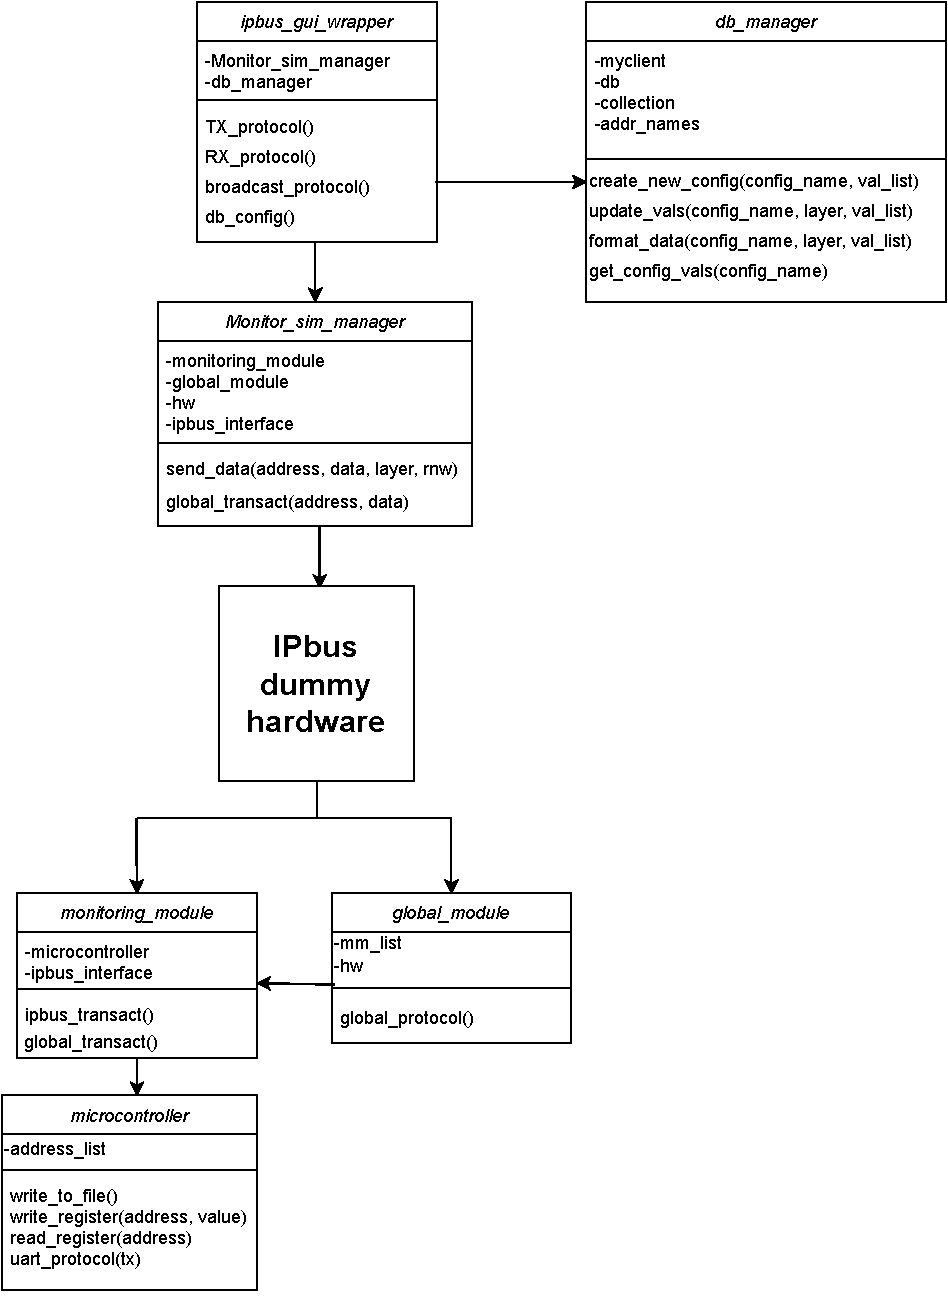
\includegraphics[width=14cm]{images/class chart.pdf}
    \caption{Class diagram of the simulation, including attributes and variables.}
    \label{fig: class_diagram}
\end{figure}
\FloatBarrier

\notinmain{snakke om i denne sectionen: features present and not present, limitations, uart communication is not simulated, fifos not simulated either, ingen FIFO. Bør eg endre simulasjonen til å lese data fra tekstfilene?}

\subsubsection{Features}

The simulation uses IPbus dummy hardware to communicate between the monitor sim manager class and the monitor module class. The dummy hardware is hosted on localhost of the computer and has the same functionality as of an IPbus module on a FPGA.  The number of layer modules and registers in the simulation is generic and can be set by the user upon instantiating the object, although the appropriate amount of modules must be manually added to the IPbus address map.

The FPGA and micro-controller class is able to perform read and write operations down to the virtual registers in the micro-controller class. The micro controller class decodes read/write bit, address and data from the TX value it is given, according to the data header discussed in \autoref{ssec: microcontroller}. A global module is also simulated, allowing for transmitting to every micro-controller by using the global transact function in the monitor sim manager. 

Using the simulation is as simple as instantiating the monitor sim manager object in the code and using the send data function to send TX data. The function will return the data from the specified RX register in IPbus. The micro-controller class will create a text file with its addresses and their contents, allowing the user to verify the data was correctly sent down to it.

The simulation was created as a platform to perform tests on IPbus code without needing the actual hardware. Halfway through the development cycle the hardware became available, and as such, the development of the simulation was not not needed. The simulation functionality is therefore outdated, but it can still be used to test simple read and write functions on software if needed.

\subsubsection{Limitations}

The simulation is built using python software and certain features is not able to be easily implemented. The USART communication protocol between the monitor module and micro-controller is omitted due to being relatively complicated to implement and for this purpose, not needed for testing GUI and API. 

The timing of data transfer is not considered in the simulations, meaning tasks such as data transfer between monitor module and micro-controller happens much faster than in the actual hardware. simulating timing is difficult to simulate using sequential code, since the actual hardware uses combinational logic that runs in parallel. We also have a prototype of the PCS chain which allows for more accurate speed tests than what a simulation could achieve. 

\subsection{Testbench}

To verify the functionality of the \gls{api}s and classes designed for the control software, testbenches have been made to test and verify the different functions. Due to the microcontroller software not being complete and not having access to the layers themselves, functions testing the entire \gls{pcs} chain has not been made, this means we do not have full coverage on the tests. Additionally, tests for the \gls{pcs}-chain is not reliable due to the high bit error rate discussed in \autoref{ssec: bit_error}.

Testing the entire system can still be done by booting up the main hub \gls{gui} and observing that the control software behaves as expected. When all parts of the \gls{dtc} is available for testing, and the bit error rate is at an acceptable level, a full scale, automatic testbench should be developed, that allows for the entire system to be quickly tested and verified. This would serve as a standard for the system and allow for quick verification when modifying or expanding existing functions.



\subsection{Test setup}
\label{ssec: test_setup}

The development of the \gls{dtc} is still undergoing and as such, we do not have access to the \gls{alpide} layers, nor do we have the necessary hardware to set up all 43 monitor boards for the \gls{pcs}. The design of the \gls{mb} is still not complete and setting up the full \gls{pcs} is therefore still not viable.

We can however set up a prototype of the \gls{pcs} that in practice, will be identical to the final product, but without connection to the actual sensors. This prototype is realized with a computer connected to the KCU105 evaluation board, and pins on the board is connected to the \gls{usart} signals. The \gls{usart} signals is then wired to a microcontroller development kit, programmed with the \gls{mb} software. An image of the prototype is shown in \autoref{fig: pcs_setup}.

\begin{figure}[!htpb]
    \centering
    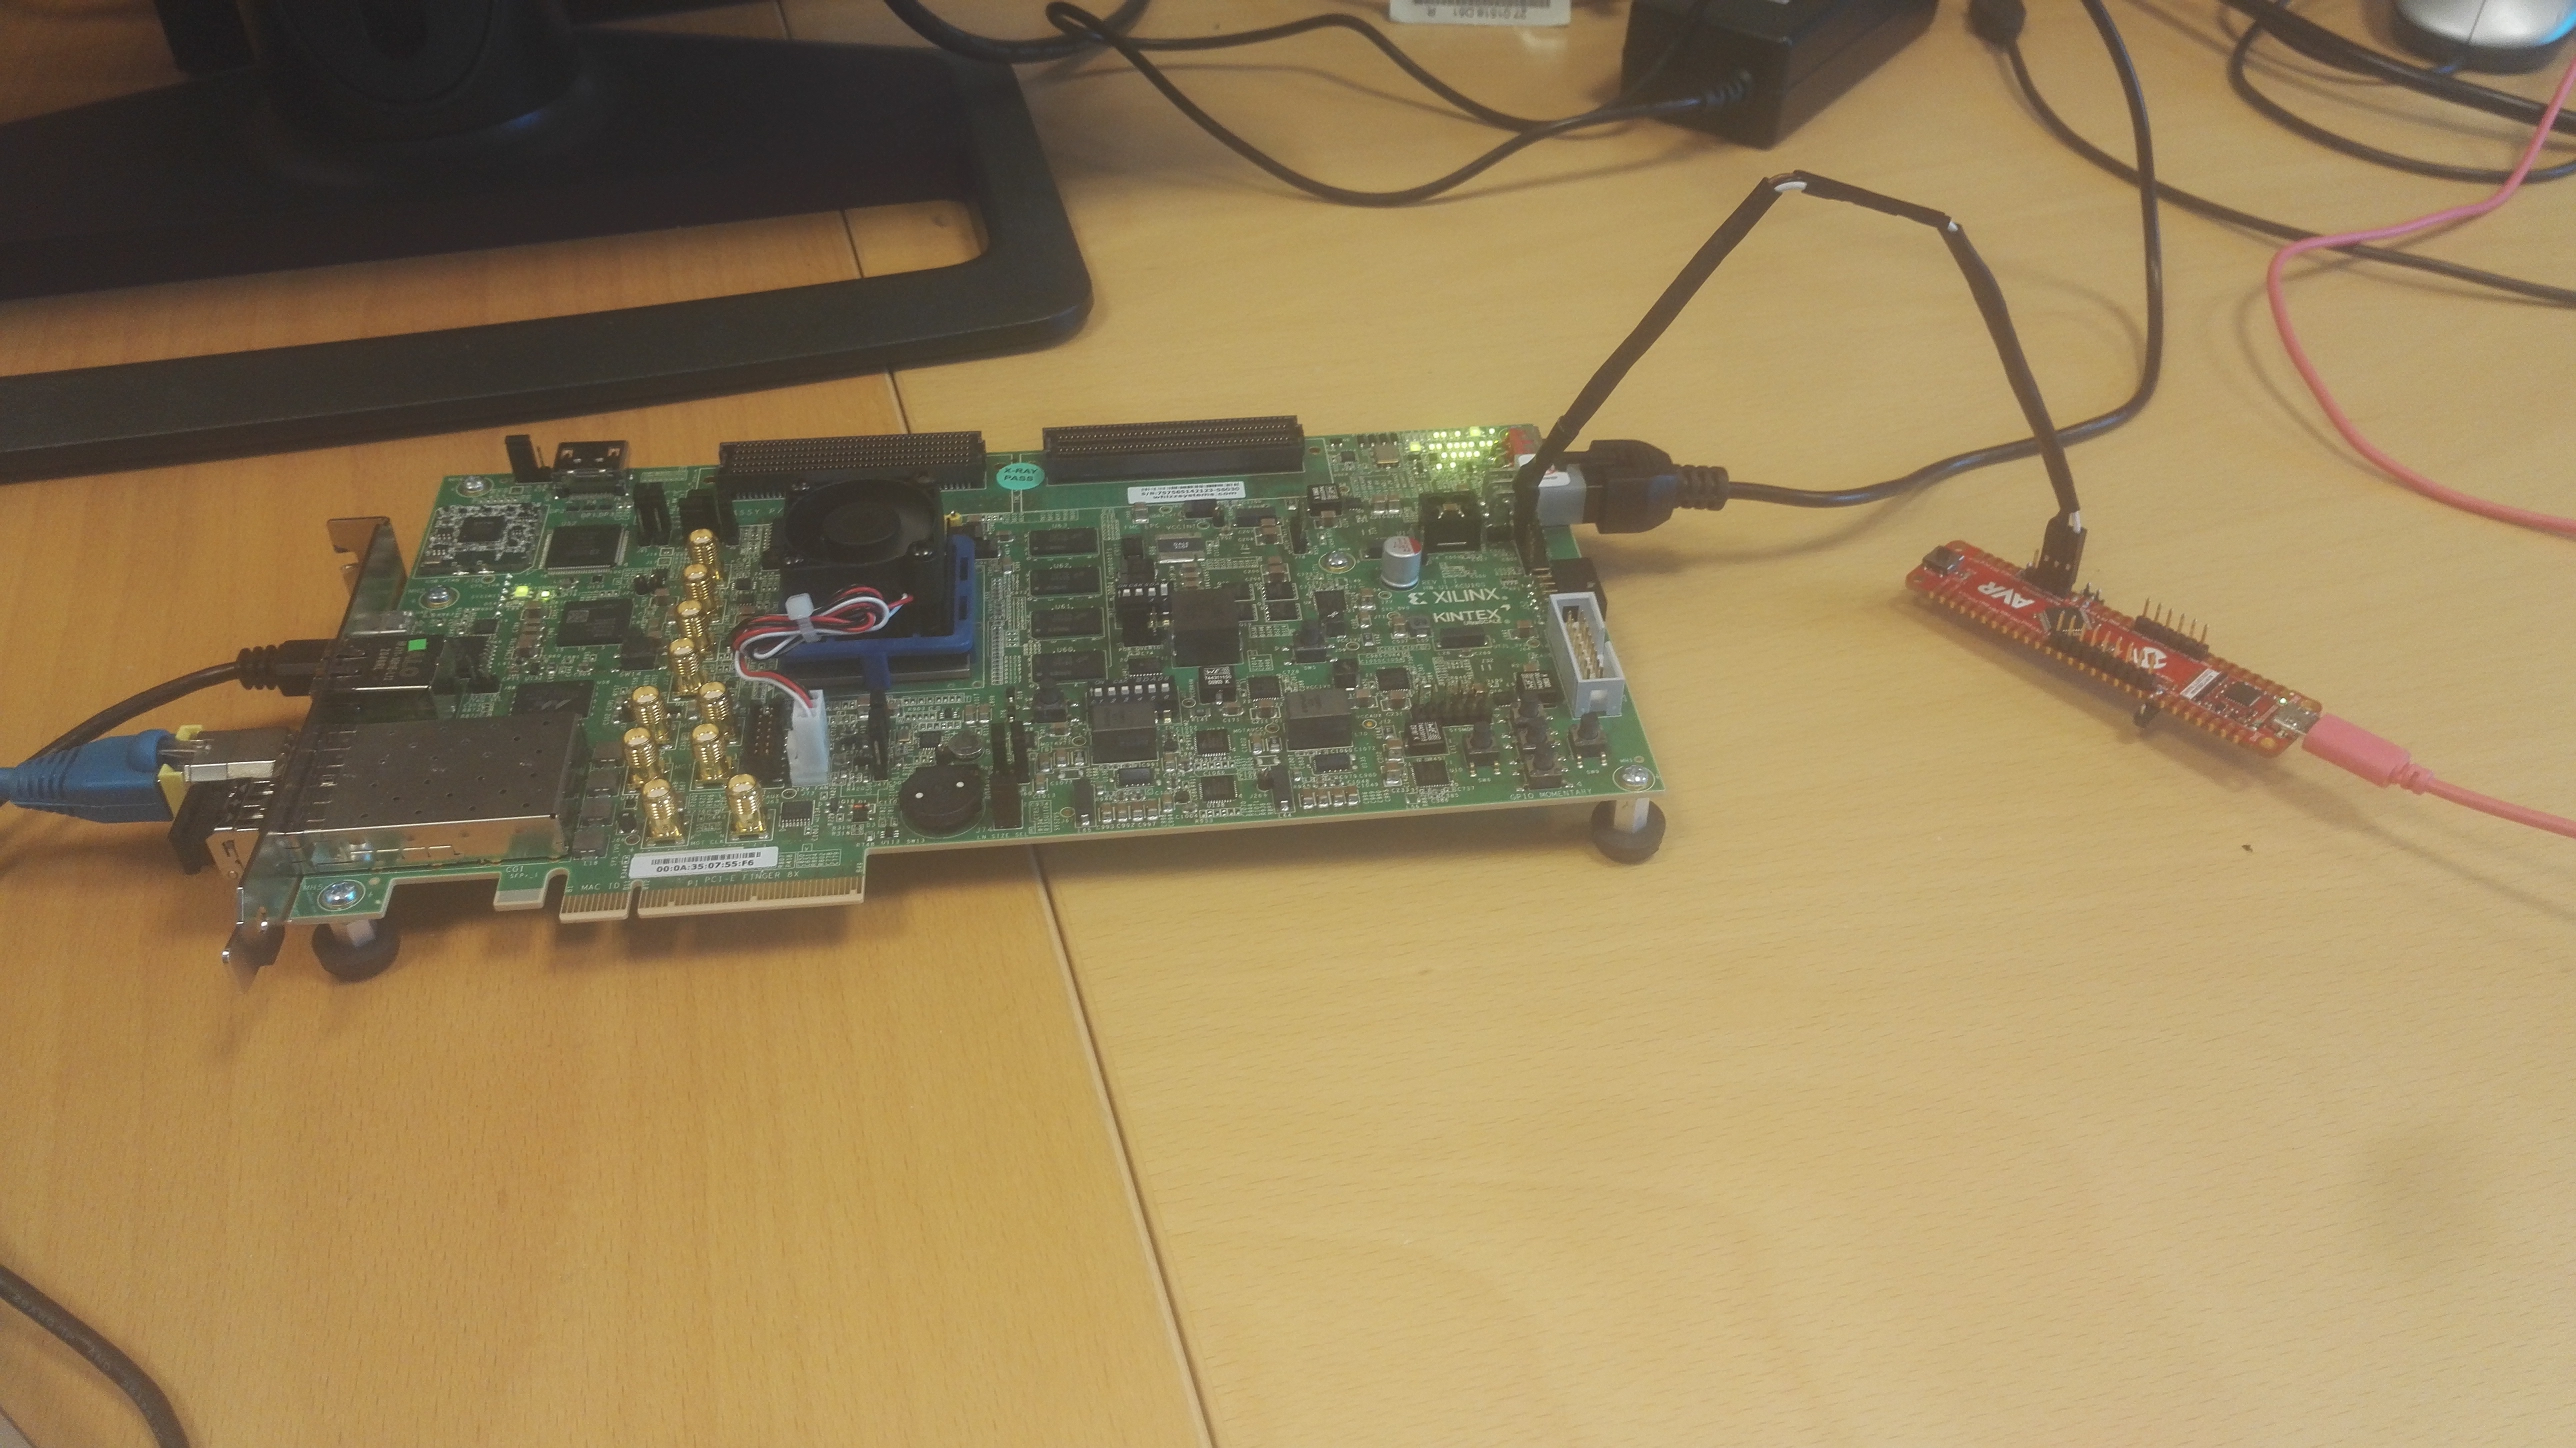
\includegraphics[width=14cm]{images/pcs_setup.jpg}
    \caption{PCS prototype setup.}
    \label{fig: pcs_setup}
\end{figure}
\FloatBarrier

The test setup can be used to test the MB Hub, and by extension, the microcontroller software. The setup also allows for verifying the two communication links in the \gls{pcs}, control software to MB Hub, and the USART communication between the MB Hub and the microcontroller.

\notinmain{The communication between the different parts of the prototype has been verified many times, but bit error rate tests that is discussed in \autoref{ssec: bit_error} shows that the reliability of the setup is inconsistent. This would suggest that this prototype should be improved or be made with more rigid components to ensure the test environment does not change over time. The fault lies between the \gls{fpga} and microcontroller so a solution could be to build a rigid connection between or put the microcontroller on an actual board to prevent it from moving. Another problem with the test setup is the wire length between the evaluation board and microcontroller. The final product will use 3 metres of wire between them, but the test setup is only about 20 cm of wire. The length of the wire determines the resistance in it, and can affect signal transmission quality. For a new test setup in the future, longer wires should be used.}


\subsection{MB Hub Verification}

The communication link between the control software and the MB Hub uses the IPbus communication protocol, and studies have shown it to be fast and reliable\cite{IPbus}. However, our communication link uses a custom \gls{fpga} design, so it must be tested to verify it works as intended.

\subsubsection{Reliability Verification}

The IPbus suite has been extensively tested, on several different boards, with no errors recorded after transmitting 10 billion packets\cite{IPbus}, but for the sake of completeness, our IPbus-link must be verified, to ensure our design is functional. The test involves reading and writing random values to a register in the MB hub, and verifying that the value read was the some one written to the register. However, we must be certain that the values are read from the actual register, and not from a buffer inside the IPbus module. To avoid this issue, the test writes and reads values from three different registers. The test reads and writes from the TX/RX registers in the dummy module, the baud rate register in the global module, and the enable register in the global module.

The test were run for 5 hours, and 10 million reads and writes were performed from each register. There were no errors reported from the communication. This suggests that the MB Hub design is reliable, and we can expect no errors to occur between the control software and the MB Hub.

\subsubsection{MB Hub Speed Test}

The transmission speed between the control software and the MB Hub can significantly impact the speed of the \gls{pcs}-chain; this property of the MB Hub must therefore be tested and verified. This communication link uses IPbus, and the IPbus user guide states that reading or writing a single word has a latency of approximately 250 $\mu$s\cite{ipbus_guide}. This number might not reflect our setup, which is why we performed a transmission speed test. The test uses the time library from Python to measure the write and read speed of the dummy module on the MB Hub.

The TX and RX register of the dummy module were written and read 1 000 000 times. On average, the single write latency was 0.4 ms($\sigma$ = 0.2 ms), and the single read latency was also 0.4 ms($\sigma$ = 0.3 ms). These measurements deviate from the assumed transmission delay of 250 $\mu$s. The imperfect time measurement from the software could be the cause of this deviation.

With this new number for the transmission delay, we can redo the timing calculations of the configuration and monitoring timing performed in \autoref{ssec: con_timing} and \autoref{eqn:monitoring_timing}, respectively. Using \autoref{eqn:one_layer_delay}, but set the IPbus delay to be 400 $\mu$s, the delay of configuring one layer becomes:

\begin{equation} \label{eqn:new_one_layer_delay}
112 * 400 + 56*33 =  46648\mu s \approx 46.6 ms
\end{equation}

A delay of 46.6 ms is closer to the measured timing of 51 ms and falls within the standard deviation of that test. There is a closer agreement with the calculations and the measurements if we consider the IPbus delay to be 400 $\mu$s. In the same vein, we can calculate the new polling timing from the monitoring process. Using \autoref{eqn:monitoring_timing} for one layer:

\begin{equation} \label{eqn:new_monitoring_timing}
8*(400\mu s + 33 \mu s + 1*400\mu s) = 6664 \mu s \approx 6.7 ms
\end{equation}

This new calculated timing for polling all data lies within the standard deviation of the measured timing of 8.7 ms. This again shows higher agreement with the calculation and the measurement if we use the measured IPbus delay.



\subsection{USART Interface Test}

\label{ssec: bit_error}
The bit error rate that occurs while sending data from the MB Hub to the microcontroller must be verified and ensured is within an acceptable rate. Testing this communication link can be done by sending data from the control software to a TX register on the MB Hub, which starts the \gls{usart}-transmission to the microcontroller. We know from previous tests the communication link between the control software and the MB Hub has a negligible error rate, we will therefore assume all bit errors to come from the communication link between the MB Hub and the microcontroller.

The test is done by performing a write to a microcontroller register, we then perform 1000 read operations from said register. This gives one sample, and this test is done a 100 000 times to give us a mean error rate. Multiple bit patterns should be used to test edge cases such as alternating bits, all 1's, all 0's or random bit pattern. Results of different bit patterns is given from \autoref{fig: all_0_bit_rate} to \ref{fig: rand_bit_rate}.

 


\begin{figure}[!ht]
    \centering
    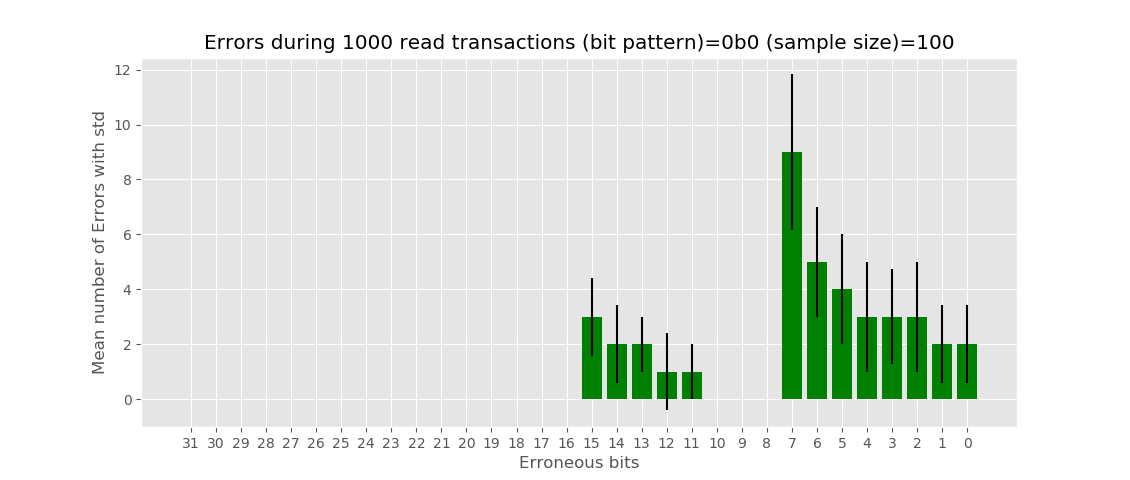
\includegraphics[width=18cm]{images/error_rate_all_0s.png}
    \caption{Histogram showing the mean bit error rate with all 0's bit pattern. Black line is the standard deviation.}
    \label{fig: all_0_bit_rate}
\end{figure}
\FloatBarrier

\begin{figure}[!ht]
    \centering
    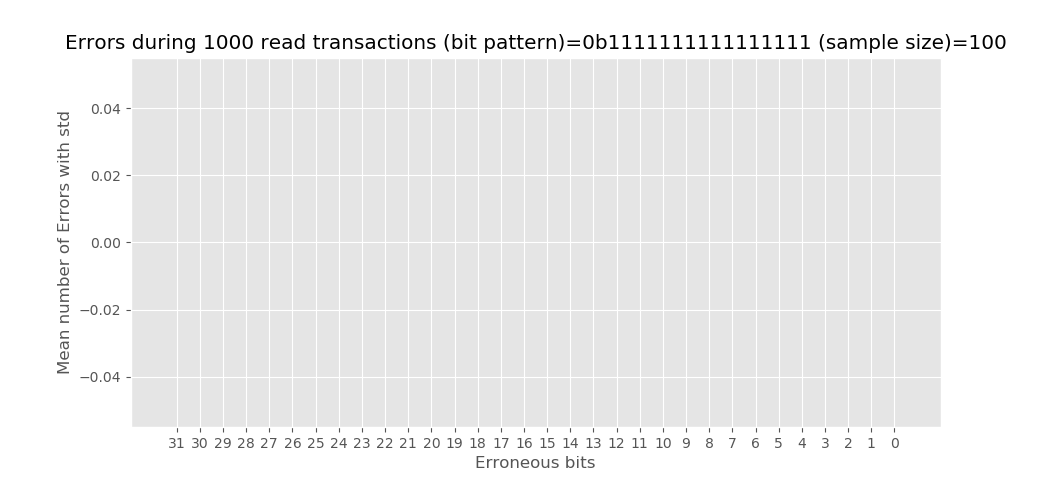
\includegraphics[width=18cm]{images/error_rate_all_1s.png}
    \caption{Histogram showing the mean bit error rate with all 1's bit pattern. Black line is the standard deviation.}
    \label{fig: all_1_bit_rate}
\end{figure}
\FloatBarrier

\begin{figure}[!ht]
    \centering
    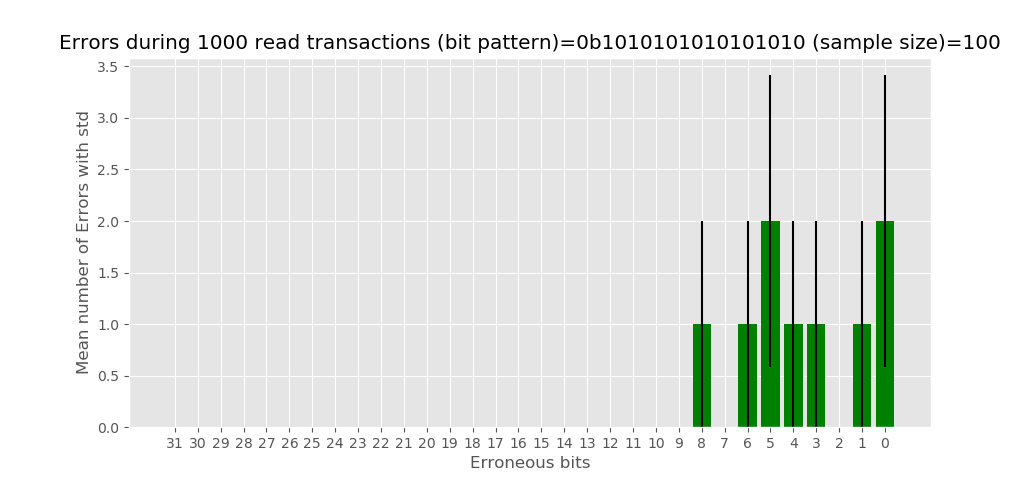
\includegraphics[width=18cm]{images/error_rate_alternating_1s.png}
    \caption{Histogram showing the mean bit error rate with alternating 1's bit pattern. Black line is the standard deviation.}
    \label{fig: alternating_1_bit_rate}
\end{figure}
\FloatBarrier

\begin{figure}[!ht]
    \centering
    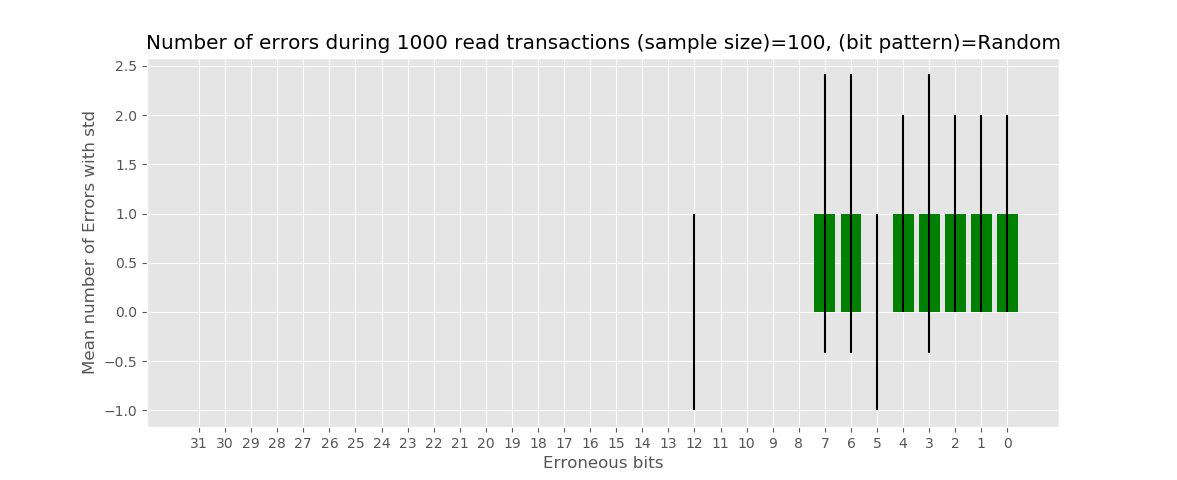
\includegraphics[width=18cm]{images/error_rate_random.png}
    \caption{Histogram showing the mean bit error rate during a random bit read operation. Black line is the standard deviation.}
    \label{fig: rand_bit_rate}
\end{figure}
\FloatBarrier

Important to note that the baud rate is set to 921600 for these tests. From the figures we can see that all but the "all 1's" test gave us errors. Alternating 1's and random bit pattern have a similar error pattern, they match well if we consider the standard deviation of the error measurements. All 0's gave a significant higher error rate than the other patterns, with worst bit error at 9 for bit 7.



The all 1's pattern is the outlier, having no errors during the entire test. That, combined with the all 0's pattern having abnormal amounts of errors, we must assume that the cause of the errors is misinterpreting 0's to be 1's. In other words, the sampling timing is not the inherent cause of the errors. Judging from the bits that have errors, only the data bits(15:0) have errors, but other than that, no obvious pattern gives us more insight into the errors.

A system's reliability can be quantified by its \gls{mtbf}, which determines the time span between faults occurring in a system\cite{mtbf_intro}. If we assume random values are being read, then from \autoref{fig: rand_bit_rate}, we can assume on average, one error occurs for every 1000 USART transactions. From \autoref{ssec: con_timing}, it was calculated that one transmission from control software to microcontroller took 288 $\mu$s, this means we can expect the \gls{mtbf} of one \gls{usart} link to be:

\begin{equation} \label{eqn:single_mtbf}
MTBF = 1000*288\mu s = 0.288 s
\end{equation}

The entire \gls{pcs}-system will have a \gls{usart}-link for every layer, which means we have to consider the \gls{mtbf} for every link to find the \gls{mtbf} for the entire system. The formula for the system \gls{mtbf} can be found by considering 43 subsystems in series\cite{mtbf_calc}. If each subsystem have the same \gls{mtbf}, then:

\begin{equation}
    \frac{1}{43*\frac{1}{MBTF}} = \frac{1}{43*\frac{1}{0.288}} = 0.0067s
\end{equation}

The \gls{mtbf} of the \gls{pcs}-system will be approximately 7 ms, which is unacceptable for use. The \gls{mtbf} of the \gls{pcs} should ideally be measured in days, not milliseconds. The conclusion from this is the \gls{usart} communication between the MB Hub and the microcontroller is unacceptable and the error rate must be significantly improved before it can be used in the \gls{pcs}.



\subsection{Baud rate error rate}

Another aspect of the \gls{pcs}-prototype that is tested is using different baud rates for the transmission between \gls{fpga} and microcontroller. If erroneous bits is caused by the sampling not hitting the falling edge of the clock, reducing the baud rate should improve the error rate, giving more time for sampling each bit. We observed in the previous section that there were an error rate of about 0.1\% for the data bits. This was tested with a baud rate of 921600. A test was performed to assess whether a lower baud rate improves the bit error rate. We can manually change the baud rate used in the transmission by writing to a register in the global module in the MB Hub. The result of the test is given in \autoref{fig: baud_error}.

\begin{figure}[!ht]
    \centering
    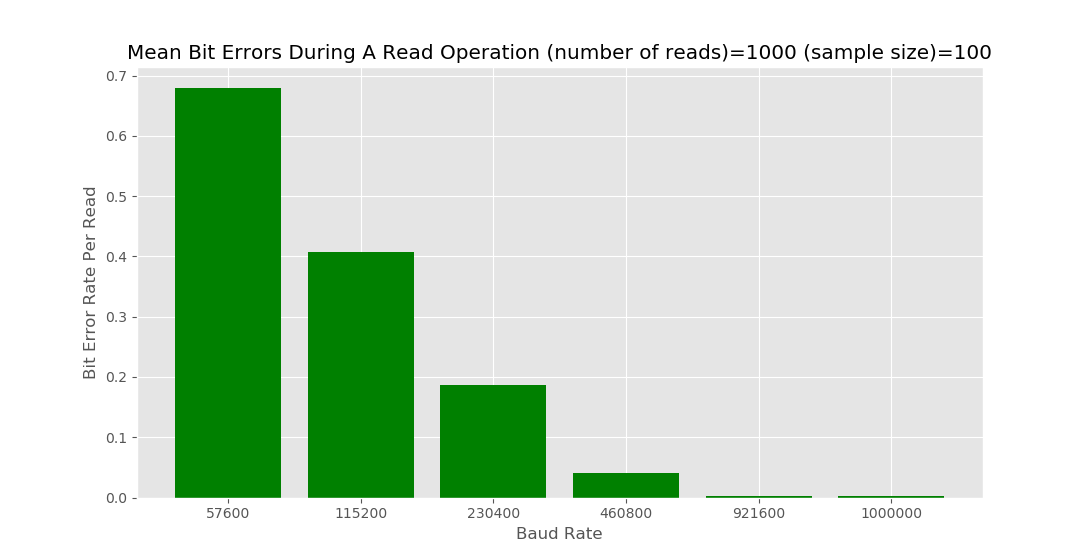
\includegraphics[width=18cm]{images/baud_error_rate.png}
    \caption{Histogram showing the amount of errors expected in one transaction for different baud rates.}
    \label{fig: baud_error}
\end{figure}
\FloatBarrier

From the figure, we can see that the lower baud rates in fact, increase the error rate, not lower it. The error rate increased from 0.1\% to a whopping 70\% on average for the lowest baud rate tested. This is an unexpected result which contradicts the behaviour of standard \gls{usart}s. The cause of this is not yet known, but an explanation for the errors can seen by observing the \gls{usart} communication with an oscilloscope. \autoref{fig: usart_com} shows the \gls{usart} communication between the microcontroller and \gls{fpga} while performing a read operation.

\begin{figure}[!ht]
    \centering
    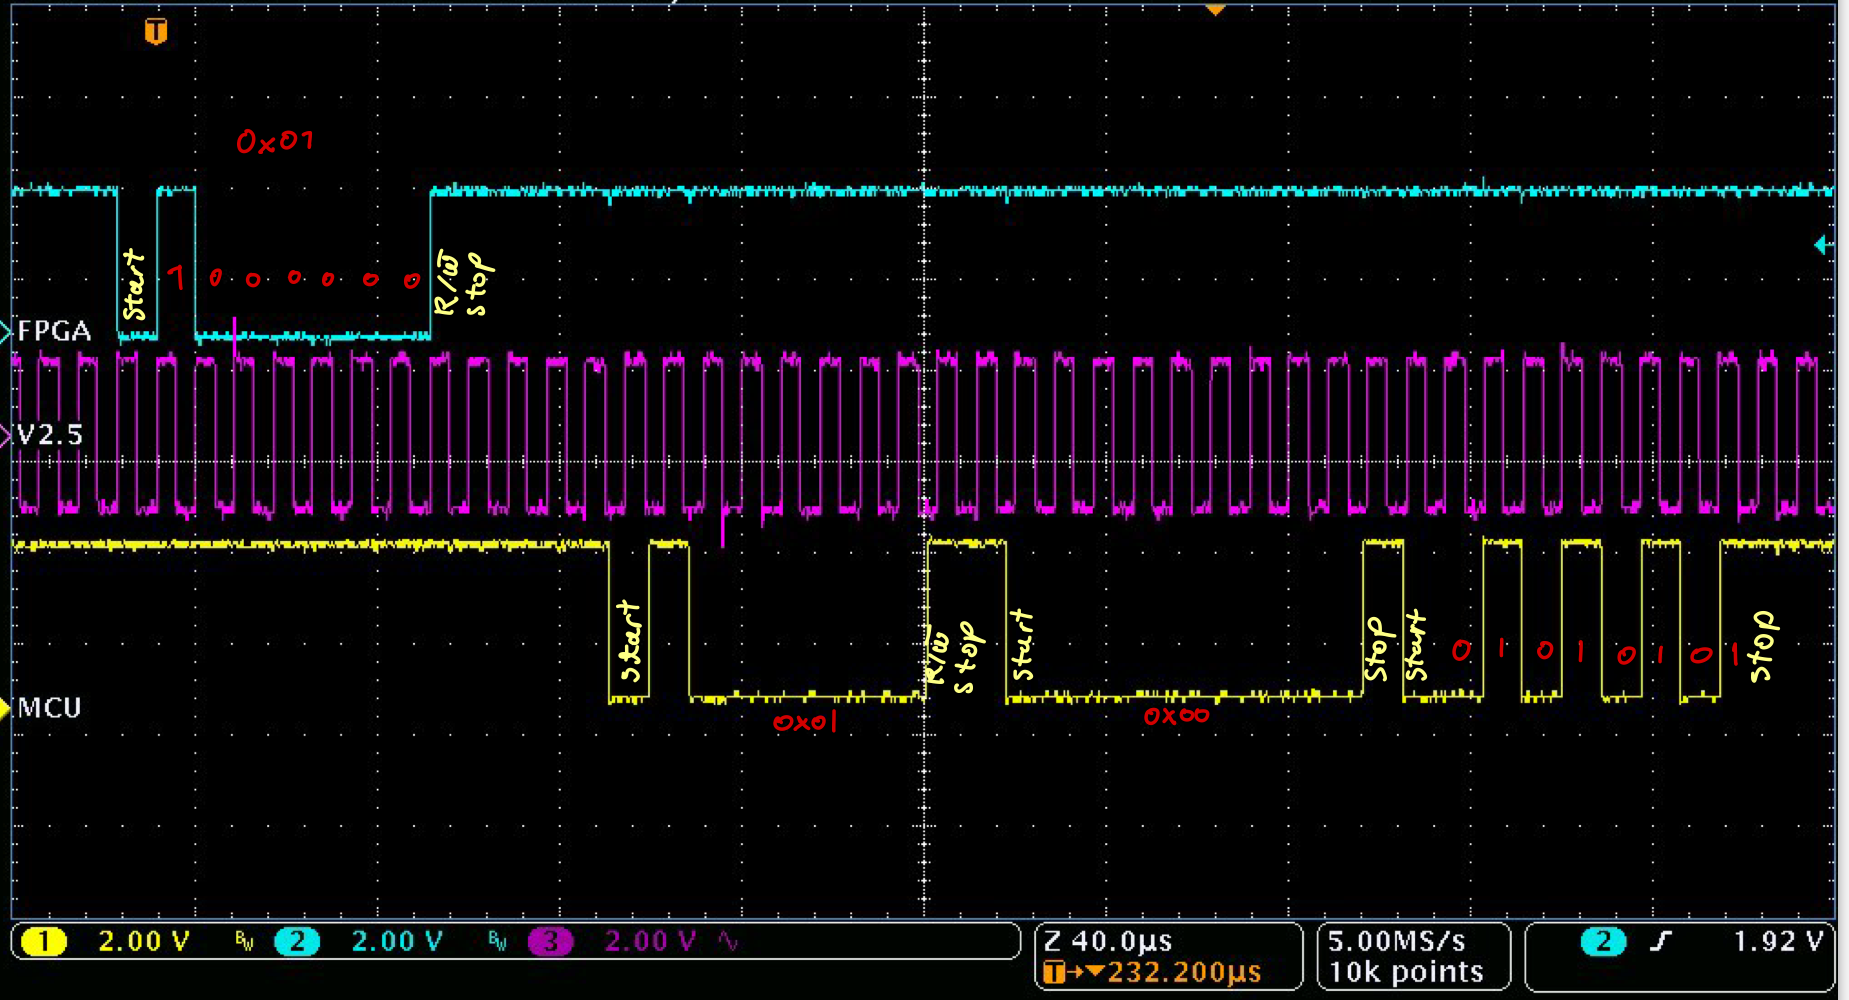
\includegraphics[width=18cm]{images/USARTTransaction.png}
    \caption{Oscilloscope image of the FPGA sending a read request to the microcontroller and receiving the data. Captured with a baud rate of 921600.}
    \label{fig: usart_com}
\end{figure}
\FloatBarrier

The figure shows the \gls{fpga} sending the read request, the microcontroller then performs a handshake by sending the read request back to the \gls{fpga}. After this it starts transmitting the data inside the two registers associated with address 0x01, which in this case is 0x00 and 0xAA. Observe from the image that the microcontroller transmits data on the falling edge of the clock, but the timing gets gradually skewed throughout the transmission. The last data bits appears to be sent from the microcontroller on the rising edge of the clock, based on the image. if the data transmission is skewed by a $\delta$t for each clock cycle, and this $\delta$t is proportional to the clock speed, then a longer clock cycle, i.e. a lower baud rate, would create more skew and result in more errors. It is recommended to capture the \gls{usart} communication at lower baud rates to observe if this deviation causes issues. This is not been done due to time constraints.

The conclusion from this is that until the underlying issue is resolved, one should use as high baud rate as possible to avoid excessive errors. The microcontroller supports baud rates up to 1 000,000 and the standard baud rate closest to it is 921600. Higher baud rates also comes with the advantage of making the transmission speed faster, which is favorable for the \gls{pcs} design.









\end{document}